%IMPAGINAZIONE DOCUMENTO
\documentclass[a4paper,11pt]{article}
\usepackage[margin=2.2cm]{geometry}

% SUPPORTO A IMPAGINAZIONE
\usepackage{lipsum}

% FONT
\usepackage[scaled]{helvet}
\usepackage[T1]{fontenc}
\renewcommand\familydefault{\sfdefault}

% CONTROLLO ORTOGRAFICO & PACCHETTI LINGUA
\usepackage[english, italian]{babel}

% TABELLE
\usepackage{tabularx}
\usepackage{booktabs}

% IMMAGINI
\usepackage{graphicx}
\graphicspath{{./diagramma/}}

% DIDASCALIE
\usepackage[labelfont={bf, small}, textfont=small]{caption}

% RIFERIMENTI IPERTESTUALI
\usepackage[colorlinks=true,
linkcolor=black,
citecolor= black,
filecolor=magenta,
urlcolor=cyan]{hyperref}

% METADATI RELAZIONE
\author{Diciotti Matteo}
\title{Relazione progetto AA 2023-2024 di\\ \textbf{Metodologie di Programmazione}}
\date{\today}

\begin{document}	
	\maketitle
	
	\subsubsection*{Dati autore}
	\begin{tabularx}{\textwidth}{l l >{\raggedleft\arraybackslash}X r}
		\textbf{Cognome} & \textbf{Nome} & \textbf{E-mail} & \textbf{Matricola}\\\toprule
		Diciotti & Matteo & matteo.diciotti@edu.unifi.it & 7072181
	\end{tabularx}
	
	\tableofcontents
	\vspace{1em}\noindent\rule{\textwidth}{2pt}
	
	\section{Presentazione progetto}
	Viene presentato nel seguito un progetto fittizio che occorre a mostrare il contesto nel quale nasce il codice sviluppato e in cui, ipoteticamente, si vorrebbe inserire.
	\subsection{Contesto: DDS} \label{fresco}
	\textbf{JDS}, ovvero \textbf{JDS is a Dispaly System}, è un software ideato per facilitare l'organizzazione di convegni, nato per accompagnare e supportare organizzatori di eventi, di una qualsiasi tipologia (non solo convegni quindi), in tutte le fasi del processo, dalla programmazione del calendario alla gestione delle prenotazioni e di eventuali pagamenti. Questo è stato progettato con l'obbiettivo di fornire una soluzione completa, gratuita e open source per la gestione e la pianificazione di eventi di ogni tipo, che si tratti di conferenze, workshop, festival o incontri sociali.\\
	Le \textbf{caratteristiche principali} del software sono:
	\begin{itemize}\setlength\itemsep{-3pt}
		\item \textbf{Gestione completa degli eventi:} Da piccoli meeting a grandi conferenze, FRESCO permette di gestire ogni aspetto dell’evento, inclusi la registrazione dei partecipanti, la pianificazione delle sessioni e la gestione delle risorse.
		\item \textbf{Interfaccia intuitiva:} Con un’interfaccia utente amichevole e facile da navigare, FRESCO rende l’organizzazione degli eventi accessibile a tutti, indipendentemente dal livello di esperienza tecnica.
		\item \textbf{Personalizzazione flessibile:} FRESCO offre ampie opzioni di personalizzazione per adattarsi alle specifiche esigenze di ogni evento, consentendo agli organizzatori di creare un’esperienza unica per i partecipanti.
		\item \textbf{Supporto della comunità:} Essendo un progetto open source, FRESCO è stato pensato per essere esteso e sostenuto interamente da una comunità di sviluppatori e organizzatori di eventi, garantendo aggiornamenti mirati e necessari dal punto di vista dei client.
		\item \textbf{Sostenibilità e accessibilità:} FRESCO è impegnato a promuovere la sostenibilità e l’accessibilità, offrendo strumenti per rendere gli eventi inclusivi e rispettosi dell’ambiente.
	\end{itemize}
	L'acrostico FRESCO vuole rappresentare la voglia di qualcosa di nuovo, qualcosa che si discosti dai più comuni programmi di organizzazione di eventi, limitando la tipica diffusione di meta-dati e aumentando la consapevolezza su tematiche critiche, spingendo l'organizzazione a valutare alternative sostenibili o raccogliendo segnalazioni qualora le opzioni non siano soddisfacenti.
	
	\subsection{Inserimento del progetto in FRESCO} \label{fresco:inserimento-elaborato}
	Il progetto presentato al punto precedente si compone di varie parti che cooperano tra loro. In questo contesto possiamo identificare il posizionamento dell'elaborato come la parte centrale del sistema per l'organizzazione di eventi, l'interno dell'architettura che modella i concetti di luogo, persona eccetera e che definisce i vincoli che sussistono tra gli oggetti. Non vengono quindi prese in considerazione nell'elaborato varie delle caratteristiche principali del progetto, come l'interfaccia per l'utilizzatore finale, il supporto della comunità o la sostenibilità, rimandando la loro implementazione e astraendo, laddove necessario, per definire un'interfaccia di funzionamento.
	
	\section{Specifiche Java}
	L'elaborato è stato implementano e testato attraverso l'utilizzo dell'IDE Eclipse, versione Linux 2024-06 (\texttt{java.verision=21.0.3}), sul sistema Kubuntu, kernel \texttt{6.8.0-38-generic} e utilizzando per questo la versione 11 di Java (\texttt{java-11-openjdk-amd64}).
	Per i test sono stati utilizzati i framework JUnit4 e AssertJ\footnote{Il framework AssertJ non è presente tra le librerie standard di Java, quindi è stato inserito come libreria aggiuntiva all'indirizzo ''\texttt{\$ROOT\_PROJECT\_DIRECTORY/test-libs/assertj-core-3.26.0.jar}'' e inserita nel buildpath del progetto Eclipse.}.
	\section{Funzionalità del progetto}
	Il progetto implementa la parte centrale del software FRESCO, come spiegato alla sezione \ref{fresco:inserimento-elaborato}. L'elaborato, in particolare, implementa il sistema che permette la generazione di nuovi eventi, l'organizzazione di questi, permettendo di recuperare il calendario contente tutti gli eventi, e la gestione delle prenotazioni agli stessi, permettendo, qualora una persona sia in dubbio se prenotarsi/pagare un evento, di osservare le modifiche che vengo apportate a questo (modifica giorno, modifica prezzo eccetera). Infine, in relazione a una convention, è possibile per ogni persona recuperare il calendario personale, che vi partecipi come uditore o come esperto. Da questa ultima affermazione risulta chiaro che ogni persona inserita è candidabile per l'assunzione in qualche evento.
	\section{Diagramma UML}
	Si mostra a fig.\ref{classdiagram} il diagramma UML delle classi senza metodi e campi, per mostrare la struttura del progetto.
	
	\begin{figure}[htb!]
		\noindent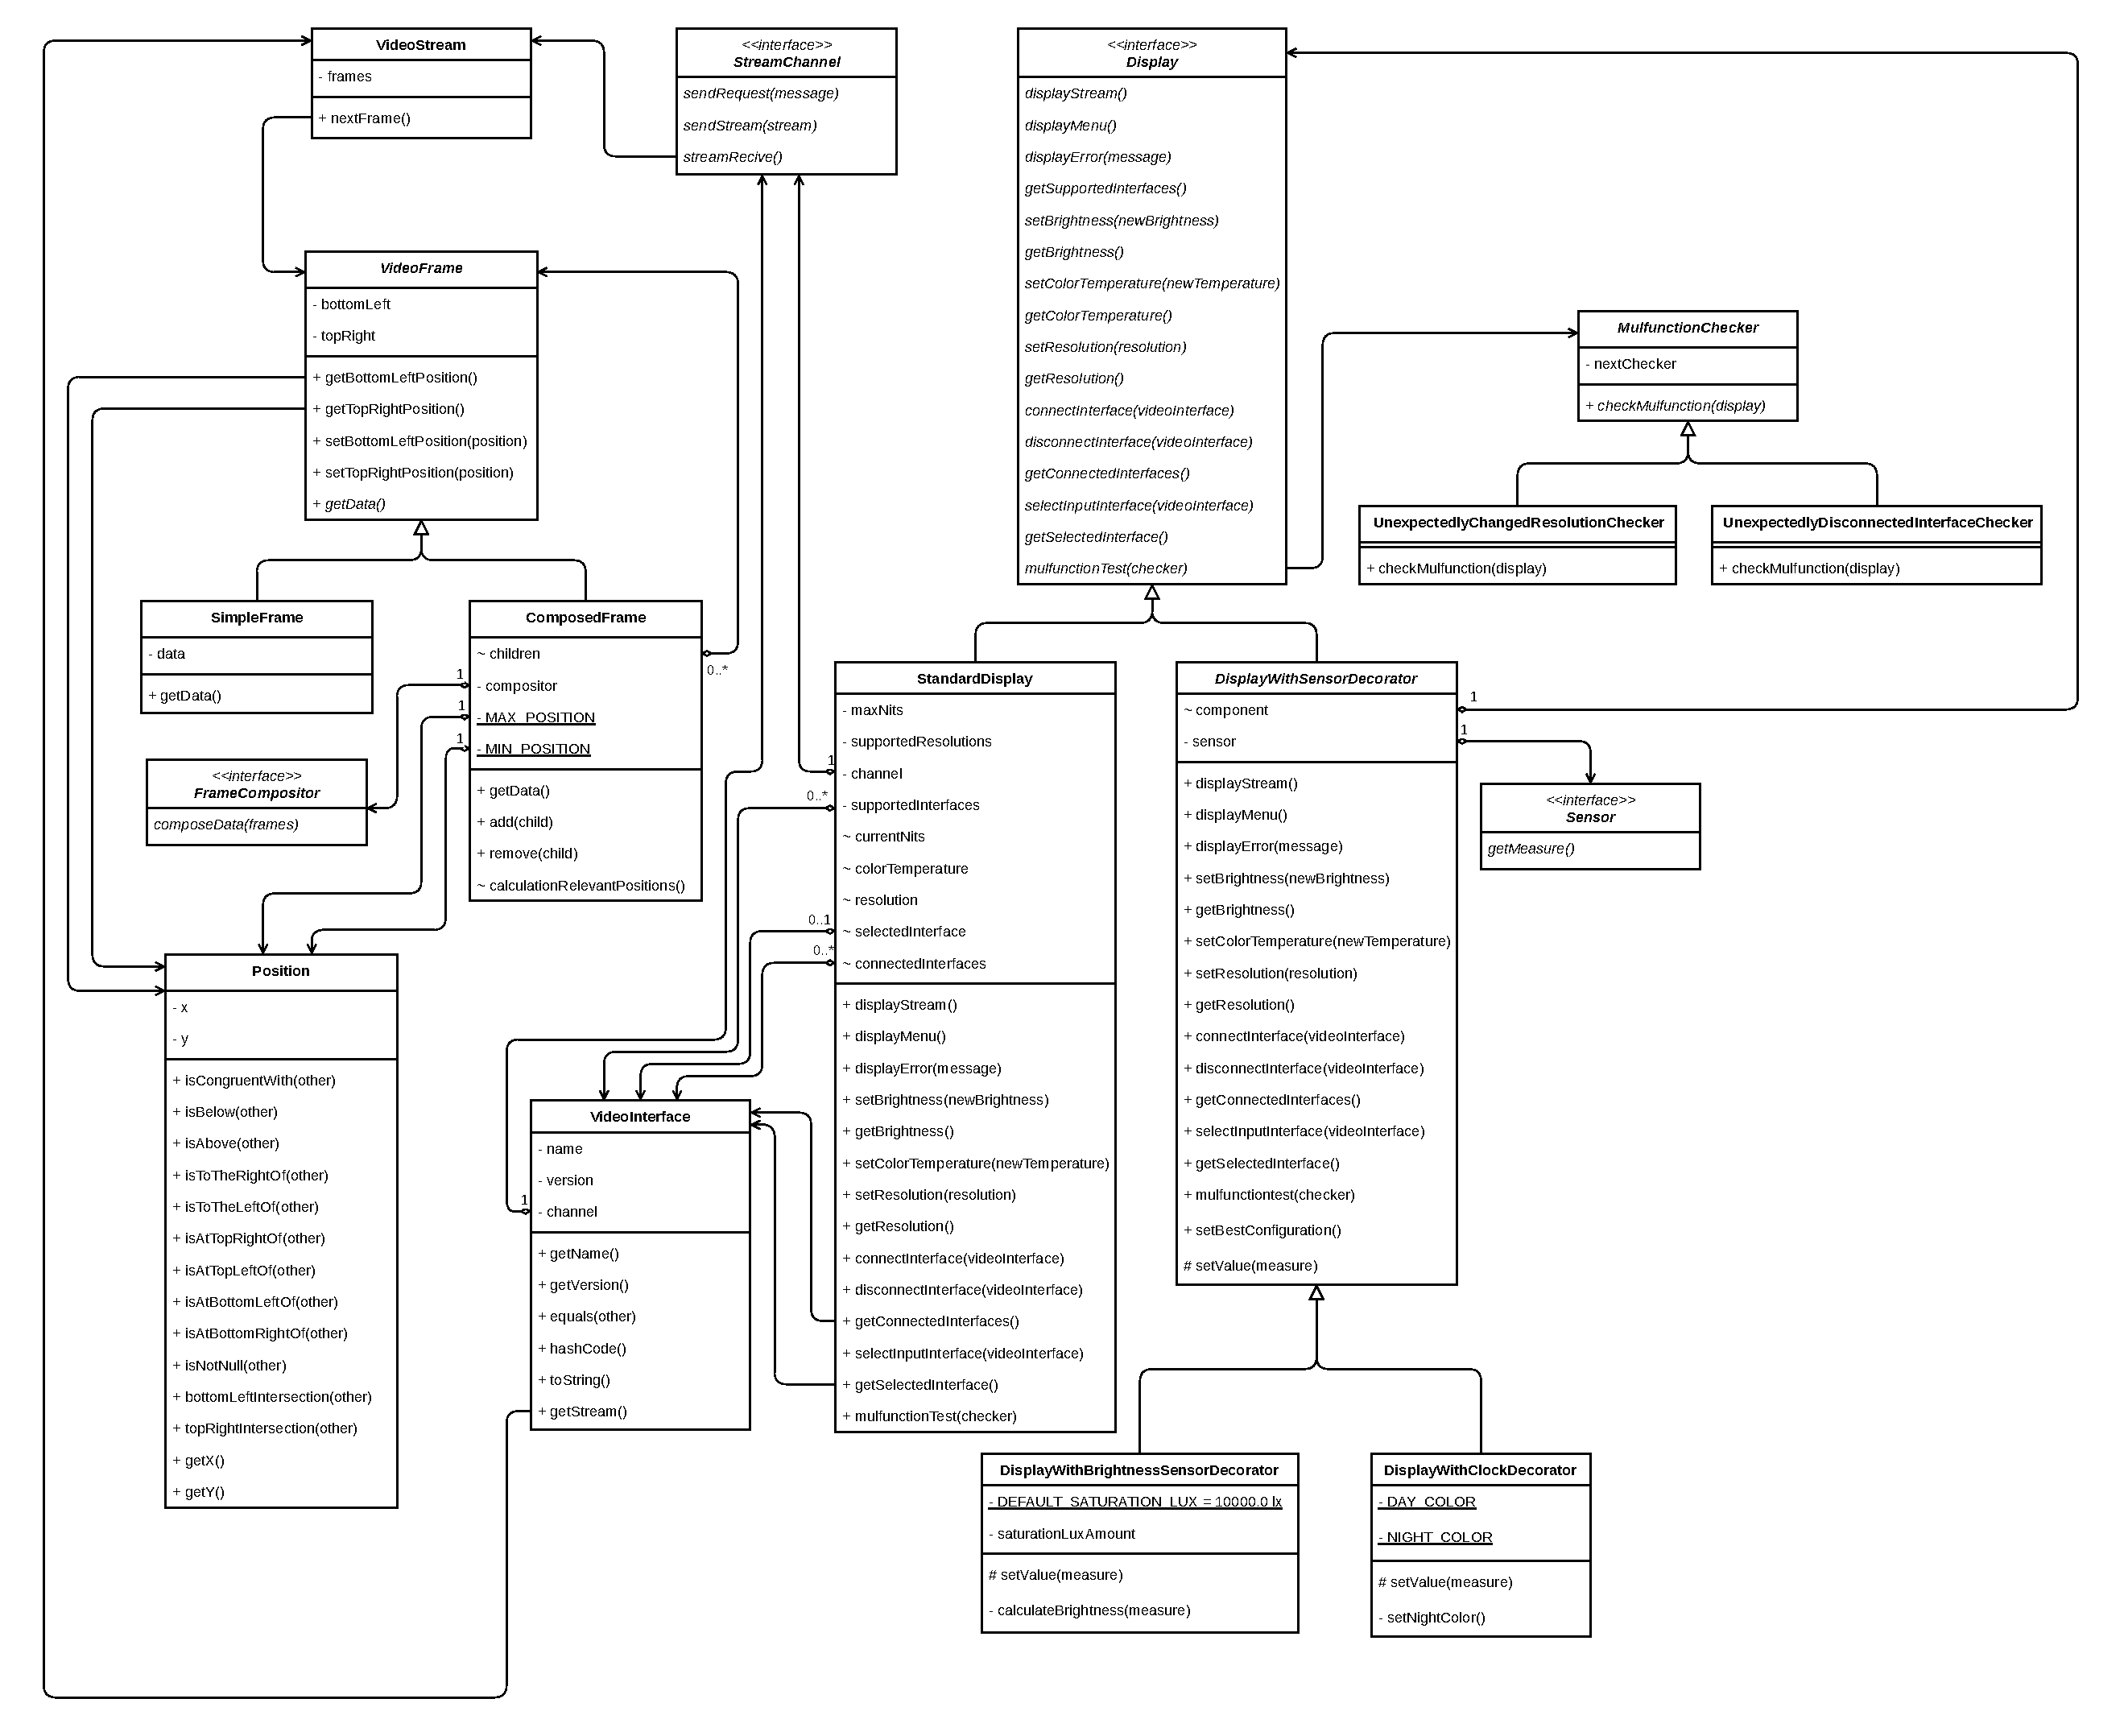
\includegraphics[width=\textwidth]{diagramma/ClassDiagramm-NoTypes.pdf}
		\captionof{figure}{Diagramma compatto delle classi descritto con \textit{Unified Modelling Lenguage}.}
		\label{classdiagram}
	\end{figure}
	\section{Lista pattern implementati}
	\begin{itemize}
		\item Observer $\rightarrow$ Persona, Event;
		% \item Decorator $\rightarrow$ StaffActivityManagerDecorator;
		\item TemplateMethod $\rightarrow$ InternalLocation::getSpecifications;
		\item FactoryMethod $\rightarrow$ CalendarGenerator::calendarOf;
		%		\item Bilder $\rightarrow$ Event; % Sarebbe utile e abbastanza fattibile
	\end{itemize}
	\section{Descrizione scelte di design}
	\section{Test}
	Si presentano nel seguito una serie di note preliminari che sono generali per tutto l'elaborato:
	\begin{itemize}\setlength\itemsep{-3pt}
		\item I test sono stati scritti in forma non completamente estesa, ovvero inserendo più asserzioni all'interno di un unico JUnitTest per controllare la correttezza di un intero metodo del \textit{Software Under Test} (o \textit{SUT}) e non il singolo comportamento di questo. È stato ritenuto che la metodologia fosse accettabile dato il contesto, in quanto vengono comunque testati separatamente i metodi del SUT, permettendo l'identificazione dell'origine dei fallimenti, ma vengono tenuti uniti i test dei vari comportamenti del singolo metodo, limitando l'eccessiva produzione di micro-JUnitTest (che generalmente sarebbe da considerare la procedura corretta).
		\item È stato deciso di non utilizzare \texttt{extractiong(String)} e \texttt{hasFieldOrPropriety(String)} (e affini), metodi di assertj, per testare lo stato di oggetti poiché questi, sebbene molto potenti, hanno il difetto di rompersi rinominando i campi, quindi venendo meno a uno dei principali utilizzi dei test.\footnote{Il metodo \texttt{org.assertj.core.api.Assertions.assertThat(.)} è deprecato solo per alcuni tipi dei parametri (si può notare dall'IDE che lo segnala contestualmente al comando di \texttt{import}). I metodi utilizzati nel progetto possiedono un nome equivalente a quello presentato ma una firma differente: questi non risultano deprecati (si può infatti notare che l'IDE non li barra direttamente nel codice). Si veda a proposito la \href{https://www.javadoc.io/doc/org.assertj/assertj-core/latest/org/assertj/core/api/Assertions.html}{documentazione del pacchetto}.}
		\item È stato ritenuto che testare i metodi auto-generati dall'IDE, ovvero getters e setters ai quali non è stata aggiunta ulteriore logica, non fosse determinante e che aumentava inutilmente la dimensione dell'elaborato. La decisione è stata presa consapevolmente che in un contesto non accademico sarebbe stato preferibile implementarli comunque.
		\item È stato preferito non testare forzatamente lo stato degli oggetti inserendo campi package-private a meno che la logica interna ai metodi non fosse particolarmente complessa per cui risultasse determinante la presenza dei test. Nei casi in cui erano presenti dei getters privi di logica sono stati utilizzati questi per testare lo stato dell'oggetto, altrimenti sono state eseguite asserzioni generiche che devono essere verificate indipendentemente dallo stato esatto dell'oggetto.
	\end{itemize}
	
	
	
\end{document}

